\chapter{Experiments}\label{chap:experiments}
Declaration files were generated for existing modules uploaded to the NPM registry. The DefinitelyTyped repository was used as a benchmark. Each one of the generated files was compared against the corresponding declaration file already uploaded to the repository.

\figref{fig:experiments-overall-funnel} shows that a declaration file was generated for 244 modules out of 6029 modules. The following sections elaborate each stage of the process and expose the reasons for generating a declaration file for only 4\% of the modules uploaded to DefinitelyTyped. Samples of the generated declaration files for templates \mintinline{text}{module}, \mintinline{text}{module-class} and \mintinline{text}{module-function} are presented in \secref{sec:experiments-declaration-files-generation}.

\definecolor{myellow}{RGB}{228,212,0}
\definecolor{mgreen}{RGB}{5,104,57}

\newcommand\funnel[3]{%
\pgfmathsetmacro\mwid{(0.3+\val*0.06)}
\pgfmathsetmacro\mradius{(\val*0.01 + 1)}
\pgfmathsetmacro\mheight{(\val*0.003 + 0.4)}
\pgfmathsetmacro\marc{\mwid-.4}
    \begin{scope}[%
        shift={(0,#1)}, 
        line width=.05pt, 
        %x=5mm, 
        %scale=1.\xi,
        yshift=\xi*4
        ]
    \draw[black,bottom color=#2, top color=#2] (-\mwid,0) -- (-\mwid+.4,-\mheight) arc (190:350:\marc cm and \mradius mm) -- (\mwid,0);
    \draw[black,fill=#3] (0,0) ellipse (\mwid cm and \mradius mm);
    \path (-\mwid,0) -- (-\mwid+.4,-\mheight) coordinate[midway] (a\xi);
    \end{scope}
}

\begin{figure}[tp]
	\hspace*{-0.28\textwidth}
	\centering
	\begin{tikzpicture}
		\foreach \val
				[%
				count=\xi starting from 0, 
				evaluate=\xi as \shadecolor using int(25*\xi),
				evaluate=\xi as \coord using int(\xi-12)
				]
			in {
				4.05,
				7.33,
				24.02,
				37.49,
				71.19,
				82.50,
				100.00
			}{
				\funnel{\coord}{mgreen!\shadecolor !myellow}{mgreen!\shadecolor !myellow}
			}   

		\node[left=0.02\textwidth of a0] {Generated Declaration Files};
		\node[right=0.07\textwidth of a0] {\textbf{244}};

		\node[left=0.02\textwidth of a1] {Run-time Information};
		\node[right=0.12\textwidth of a1] {\textbf{442}};

		\node[left=0.02\textwidth of a2] {Working Examples};
		\node[right=0.26\textwidth of a2] {\textbf{1448}};

		\node[left=0.02\textwidth of a3] {Code Examples};
		\node[right=0.38\textwidth of a3] {\textbf{2260}};

		\node[left=0.02\textwidth of a4] {README file};
		\node[right=0.70\textwidth of a4] {\textbf{4292}};

		\node[left=0.02\textwidth of a5] {Github Repository};
		\node[right=0.80\textwidth of a5] {\textbf{4974}};

		\node[align=right,left=0.02\textwidth of a6, text width=0.25\textwidth] {Definitely Typed Modules};
		\node[right=0.97\textwidth of a6] {\textbf{6029}};

	\end{tikzpicture}
	\caption[Number of analyzed modules for each stage of the experiment]{\textbf{Number of analyzed modules for each stage of the experiment} - A TypeScript Declaration File was generated for only 244 modules, out of 6029 modules in the DefinitelyTyped Repository. It was possible to gather valid run-time information for only 25\% of the modules for which a Code Example was extracted.}
	\label{fig:experiments-overall-funnel}
\end{figure}

Finally, an analysis on the usage of JavaScript operators can be seen in \secref{sec:experiments-js-operators-usage}. The goal is to gather empirical evidence that shows which are the most common types that developers use with every JavaScript operator.

\section{Definitely Typed Benchmark}

\subsection{Code Examples}
Retrieving the code examples from the JavaScript libraries' repositories proved to be a pragmatic way of capturing the types. However, as shown in \figref{fig:experiments-overall-funnel}, working code examples for only 2260 modules could be retrieved. The process of getting a valid code example for a module is divided in 4 blocks:
\begin{itemize}
	\item Extracting repositories url.
	\item Extracting readme files.
	\item Extracting code examples within readme files.
	\item Executing code examples and discarding failing ones.
\end{itemize}

The results obtained for each on of them are described in the following sections.

\subsubsection{Repositories URL}
The url of the repositories could be retrieved for only 4974 modules. More than 1000 modules do not have the repository entry in their corresponding \mintinline{text}{package.json} files. Therefore, the \mintinline{text}{npm view <module> repository.url} command returns an empty value. This is even happening for important modules like \mintinline{text}{ace}.

\subsubsection{Readme Files}
700 modules simply do not have a readme file in their repositories. The implementation does contemplate, however, different naming conventions like \mintinline{text}{readme.md} or \mintinline{text}{README.md}.

\subsubsection{Code Examples Extraction}
The 50\% loss is mainly explained because developers did not wrap their code around a block using the \mintinline{text}{javascript} or \mintinline{text}{js} tags. As explained in \secref{sec:conclusions-future-work}, the process of extracting code examples from a repository can be greatly improved. However, counting with code examples for 2200 modules was considered to be enough for evaluating the generation of declaration files.

\subsubsection{Code Examples Execution}
The 2260 extracted code examples were executed by installing the required packages and running the code as a \mintinline{text}{node} application. Working and functional code examples could only be extracted for 1448 modules. 812 modules did not run correctly and were discarded. Some failing samples were analyzed and there were mainly two reasons for the failure:
\begin{enumerate}
	\item The code example had been properly extracted but the code itself was not working. It was executing the library in an unsupported way, hence the error at run-time.
	\item The extracted code example was not intended to be executed or it was not even valid JavaScript code.
\end{enumerate}

Improving the retrieval of code examples for a specific module will definitely have a positive impact in this number.

\subsection{Run-time Information Gathering} \label{sec:experiments-run-time-information-gathering}
Run-time information could only be extracted for 442 modules out of 1448 modules with working code examples. As explained in \secref{sec:run-time-wrapper-objects}, the behavior of the code under analysis was explicitly modified by wrapping the arguments around Wrapper Objects. It definitely had an influence on some modules by causing run-time errors when executing the code examples. Furthermore, Jalangi's instrumentation itself caused some executions to fail, since the modules contained JavaScript features that are not supported by Jalangi. As a result, these modules could not be executed.

An instrumentation without user defined analysis modules was not applied to the 1448 working code examples. Therefore, it was not possible to determine which modules were failing only because of Jalangi's own limitations.

\subsection{Declaration Files Generation} \label{sec:experiments-declaration-files-generation}
Finally, a declaration file was generated for 244 modules. Despite the correct execution of instrumented code examples, some of the 442 modules mentioned in \secref{sec:experiments-run-time-information-gathering} did not contain suitable run-time information for generating a declaration file. 198 of the extracted code examples did not execute the library itself and therefore the collected run-time information was not useful for generating a declaration file.

\subsubsection{Results}
The following section exhibits some samples of the 244 generated declaration files.  It shows some results for each of the implemented templates: \mintinline{text}{module}, \mintinline{text}{module-function} and \mintinline{text}{module-class}.

\figref{fig:experiments-results-module-function} shows the generated declaration files for simple modules like \mintinline{text}{abs}, \mintinline{text}{dirname-regex} and \mintinline{text}{escape-html}. All of them were generated using the \mintinline{text}{module-function} template. There are no differences between the generated files and the corresponding declaration files uploaded to DefinitelyTyped.

Templates of type \mintinline{text}{module-class} are shown for modules \mintinline{text}{flake-idgen}, \mintinline{text}{route-parser} and \mintinline{text}{timer-machine} in \figref{fig:experiments-results-module-class-flake-idgen}, \figref{fig:experiments-results-module-class-route-parser} and \figref{fig:experiments-results-module-class-timer-machine}, respectively. Properties of interfaces and class methods are correctly generated. Optional parameters are not detected, as it was not considered for the implementation.

Finally, \mintinline{text}{module} template is presented for \mintinline{text}{is-uuid} module in \figref{fig:experiments-results-module-is-uuid}.

It is worth mentioning that for some libraries the declaration file in DefinitelyTyped was not correct. For example, for \mintinline{text}{datadog-metrics}, some properties of an interface were included in the generated declaration file but they were not present in the one in DefinitelyTyped. However, as shown in \figref{fig:experiments-results-module-datadog-metrics}, the properties are indeed used in the source code and should be included. The limitations of using DefinitelyTyped as a baseline for comparison are explained in detail in \chapref{chap:conclusion}.

\begin{figure}[tp]
	\centering
	\begin{lrbox}{\mintedbox}
		\begin{minipage}{0.49\textwidth}
			\tscode{code/experiments/results/module-function/abs/generated.d.ts}
		\end{minipage}
	\end{lrbox}
	\subfloat[abs/index.d.ts - Generated]{\usebox{\mintedbox}}
	\hfill
	\begin{lrbox}{\mintedbox}
		\begin{minipage}{0.49\textwidth}
			\tscode{code/experiments/results/module-function/abs/definitely-typed.d.ts}
		\end{minipage}
	\end{lrbox}
	\subfloat[abs/index.d.ts - DefinitelyTyped]{\usebox{\mintedbox}}

	\begin{lrbox}{\mintedbox}
		\begin{minipage}{0.49\textwidth}
			\tscode{code/experiments/results/module-function/dirname-regex/generated.d.ts}
		\end{minipage}
	\end{lrbox}
	\subfloat[dirname-regex/index.d.ts - Generated]{\usebox{\mintedbox}}
	\hfill
	\begin{lrbox}{\mintedbox}
		\begin{minipage}{0.49\textwidth}
			\tscode{code/experiments/results/module-function/dirname-regex/definitely-typed.d.ts}
		\end{minipage}
	\end{lrbox}
	\subfloat[dirname-regex/index.d.ts - DefinitelyTyped]{\usebox{\mintedbox}}

	\begin{lrbox}{\mintedbox}
		\begin{minipage}{0.49\textwidth}
			\tscode{code/experiments/results/module-function/escape-html/generated.d.ts}
		\end{minipage}
	\end{lrbox}
	\subfloat[escape-html/index.d.ts - Generated]{\usebox{\mintedbox}}
	\hfill
	\begin{lrbox}{\mintedbox}
		\begin{minipage}{0.49\textwidth}
			\tscode{code/experiments/results/module-function/escape-html/definitely-typed.d.ts}
		\end{minipage}
	\end{lrbox}
	\subfloat[escape-html/index.d.ts - DefinitelyTyped]{\usebox{\mintedbox}}

	\caption[Module-function results]{\textbf{Module-function results} - Results are shown for modules \mintinline{text}{abs}, \mintinline{text}{dirname-regex}, \mintinline{text}{escape-html}. On the left side the generated declaration file with \mintinline{text}{dts-generate}. On the right side the corresponding file in the DefinitelyTyped repository. Functions are correctly detected and input types are accurately inferred. Both files are parsed for comparison, as explained in \secref{sec:approach-parsing}. Therefore, subtle differences in the syntax between both files are not important.}
	\label{fig:experiments-results-module-function}
\end{figure}

\begin{figure}[tp]
	\centering
	\begin{lrbox}{\mintedbox}
		\begin{minipage}{0.8\textwidth}
			\tscode{code/experiments/results/module-class/flake-idgen/generated.d.ts}
		\end{minipage}
	\end{lrbox}
	\subfloat[flake-idgen/index.d.ts - Generated]{\usebox{\mintedbox}}

	\begin{lrbox}{\mintedbox}
		\begin{minipage}{0.8\textwidth}
			\tscode{code/experiments/results/module-class/flake-idgen/definitely-typed.d.ts}
		\end{minipage}
	\end{lrbox}
	\subfloat[flake-idgen/index.d.ts - DefinitelyTyped]{\usebox{\mintedbox}}

	\caption[Module-class results | flake-idgen]{\textbf{Module-class results | flake-idgen} - Parameters of interface \mintinline{text}{ConstructorOptions} are correctly detected. Name of interface differs since it is automatically generated based on the name of the argument variable. Optional properties were not implemented, hence the \mintinline{text}{undefined} type for some properties. Analogously, callback \mintinline{text}{cb} is inferred as \mintinline{text}{undefined}.}
	\label{fig:experiments-results-module-class-flake-idgen}
\end{figure}

\begin{figure}[tp]
	\centering
	\begin{lrbox}{\mintedbox}
		\begin{minipage}{0.8\textwidth}
			\tscode{code/experiments/results/module-class/route-parser/generated.d.ts}
		\end{minipage}
	\end{lrbox}
	\subfloat[route-parser/index.d.ts - Generated]{\usebox{\mintedbox}}

	\begin{lrbox}{\mintedbox}
		\begin{minipage}{0.8\textwidth}
			\tscode{code/experiments/results/module-class/route-parser/definitely-typed.d.ts}
		\end{minipage}
	\end{lrbox}
	\subfloat[route-parser/index.d.ts - DefinitelyTyped]{\usebox{\mintedbox}}

	\caption[Module-class results | route-parser]{\textbf{Module-class results | route-parser} - Constructor and methods are correctly identified. Specific signature of dictionary \mintinline{text}{params} is not detected. Instead, a generic \mintinline{text}{object} is inferred.}
	\label{fig:experiments-results-module-class-route-parser}
\end{figure}

\begin{figure}[tp]
	\centering
	\begin{lrbox}{\mintedbox}
		\begin{minipage}{0.8\textwidth}
			\tscode{code/experiments/results/module-class/timer-machine/generated.d.ts}
		\end{minipage}
	\end{lrbox}
	\subfloat[timer-machine/index.d.ts - Generated]{\usebox{\mintedbox}}

	\begin{lrbox}{\mintedbox}
		\begin{minipage}{0.8\textwidth}
			\tscode{code/experiments/results/module-class/timer-machine/definitely-typed.d.ts}
		\end{minipage}
	\end{lrbox}
	\subfloat[timer-machine/index.d.ts - DefinitelyTyped]{\usebox{\mintedbox}}

	\caption[Module-class results | timer-machine]{\textbf{Module-class results | timer-machine} - Parameter \mintinline{text}{started} is inferred as \mintinline{text}{undefined} instead of marking it as optional. Methods that were not executed do not appear in the generated declaration file.}
	\label{fig:experiments-results-module-class-timer-machine}
\end{figure}

\begin{figure}[tp]
	\centering
	\begin{lrbox}{\mintedbox}
		\begin{minipage}{0.8\textwidth}
			\tscode{code/experiments/results/module/is-uuid/generated.d.ts}
		\end{minipage}
	\end{lrbox}
	\subfloat[is-uuid/index.d.ts - Generated]{\usebox{\mintedbox}}

	\begin{lrbox}{\mintedbox}
		\begin{minipage}{0.8\textwidth}
			\tscode{code/experiments/results/module/is-uuid/definitely-typed.d.ts}
		\end{minipage}
	\end{lrbox}
	\subfloat[is-uuid/index.d.ts - DefinitelyTyped]{\usebox{\mintedbox}}

	\caption[Module results | is-uuid]{\textbf{Module results | is-uuid} - Methods that were not executed are not included in the declaration file.}
	\label{fig:experiments-results-module-is-uuid}
\end{figure}

\begin{figure}[tp]
	\centering
	\begin{lrbox}{\mintedbox}
		\begin{minipage}{0.49\textwidth}
			\tscode{code/experiments/results/module/datadog-metrics/generated.d.ts}
		\end{minipage}
	\end{lrbox}
	\subfloat[datadog-metrics/index.d.ts - Generated]{\usebox{\mintedbox}}
	\hfill
	\begin{lrbox}{\mintedbox}
		\begin{minipage}{0.49\textwidth}
			\tscode{code/experiments/results/module/datadog-metrics/definitely-typed.ts}
		\end{minipage}
	\end{lrbox}
	\subfloat[datadog-metrics/index.d.ts - DefinitelyTyped]{\usebox{\mintedbox}}

	\begin{lrbox}{\mintedbox}
		\begin{minipage}{0.95\textwidth}
			\tscode{code/experiments/results/module/datadog-metrics/logger-datadog-metrics.js}
		\end{minipage}
	\end{lrbox}
	\subfloat[datadog-metrics/logger.js]{\usebox{\mintedbox} \label{fig:subfloat-datadog-logger} }

	\caption[Missing properties | datadog-metrics]{\textbf{Missing properties | datadog-metrics} - Properties \mintinline{text}{aggregator} and \mintinline{text}{reporter} are not in the DefinitelyTyped version, but they appear in the generated declaration file. However, they are indeed used by the library, as exposed in lines 2 and 3 of the library's source code shown in \protect\subref{fig:subfloat-datadog-logger}.}
	\label{fig:experiments-results-module-datadog-metrics}
\end{figure}

\subsection{Evaluation}
As shown in \figref{fig:experiments-typescript-templates-distribution-definitely-typed}, 20\% of the declaration files in DefinitelyTyped are written using the \mintinline{text}{module-function}. However, 57\% of the 244 generated declaration files are written with the \mintinline{text}{module-function} template. Additionally, the complexity of evaluating declaration files written with the \mintinline{text}{module-function} is considerably lower than for other templates. The evaluation for templates \mintinline{text}{module-class} and \mintinline{text}{module} was not implemented.

33 out of 116 evaluated modules have no difference with their corresponding declaration file in DefinitelyTyped.

\begin{figure}[tp]
	\centering
	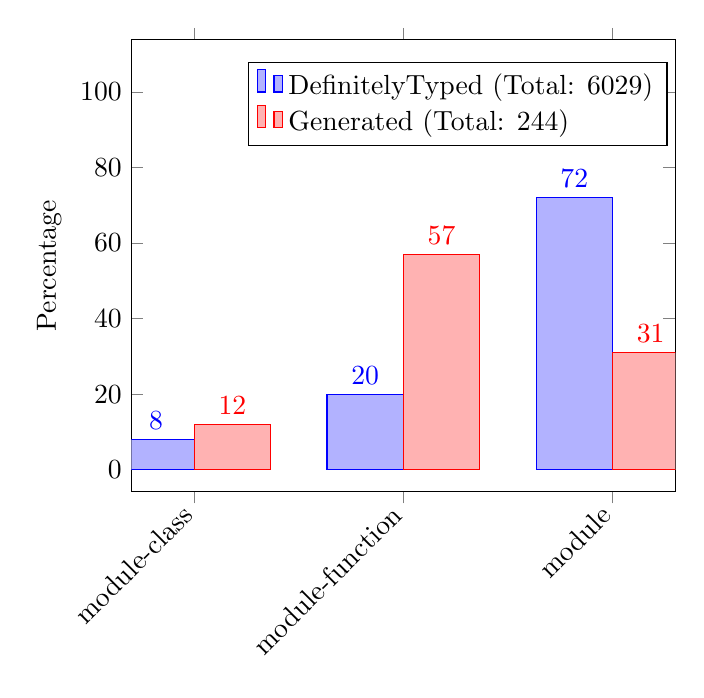
\begin{tikzpicture}
		\begin{axis}[
			ybar,
			width=0.7\textwidth,
			ybar=0pt,
			ymax=100,
			enlargelimits=0.15,
			bar width=0.08\textwidth,
			legend columns=1,
			legend cell align={left},
			legend style={at={(0.6,0.95)}, anchor=north},
			symbolic x coords={module-class,module-function,module},
			xtick=data,
			ylabel=Percentage,
			nodes near coords, 
			nodes near coords align={vertical},
			x tick label style={rotate=45,anchor=east},
		]
		\addplot coordinates {
			(module-class, 8)
			(module-function, 20)
			(module, 72)
		};

		\addplot coordinates {
			(module-class, 12)
			(module-function, 57)
			(module, 31)
		};
		\legend{DefinitelyTyped (Total: 6029), Generated (Total: 244)}
		\end{axis}
	\end{tikzpicture}

	\caption[TypeScript templates distribution | Generated \& DefinitelyTyped]{\textbf{TypeScript templates distribution | Generated \& DefinitelyTyped} - Out of a total of 6029, 72\% of the modules uploaded to the DefinitelyTyped repository use the \mintinline{text}{module} template and only 20\% use the \mintinline{text}{module-function} one. However, 57\% of the 244 generated declaration files use the \mintinline{text}{module-function} template.
	}

	\label{fig:experiments-typescript-templates-distribution-definitely-typed}
\end{figure}

\section{JavaScript Operators Usage} \label{sec:experiments-js-operators-usage}
The following section presents a study on the usage of JavaScript operators. The types of the operands of each operator were recorded with Jalangi. The goal is to better understand how developers are using JavaScript operators and what they expect from them. The study was performed on the 442 modules used for gathering the run-time information, as shown in \figref{fig:experiments-overall-funnel}.

The results might have exposed unexpected development patterns like multiplying a \mintinline{text}{function} and an \mintinline{text}{object}. Conversely, the obtained results support the idea that developers are using operators in a traditional way, despite the possibility in JavaScript of using any type with any operator. 

Table \ref{table:experiments-number-of-events-per-operator} summarizes the distribution of events per operator. In total, 1263866 events were collected.

The most relevant results are presented in the following sections.

\begin{table}[tp]
	\centering

	\begin{tabular}{ |c|c|c| } 
		\hline
		\textbf{Operator} & \multicolumn{2}{|c|}{\textbf{Number of events}} \\
		\hline
		\mintinline{text}{<} & 143666 & 11.37\% \\
		\mintinline{text}{>} & 8914 & 0.71\% \\
		\mintinline{text}{<=} & 2537 & 0.20\% \\
		\mintinline{text}{>=} & 1835 & 0.15\% \\
		\mintinline{text}{instanceof} & 1823 & 0.14\% \\
		\mintinline{text}{in} & 2242 & 0.18\% \\
		\mintinline{text}{+} & 261669 & 20.70\% \\
		\mintinline{text}{-} & 196598 & 15.56\% \\
		\mintinline{text}{*} & 82821 & 6.55\% \\
		\mintinline{text}{/} & 318 & 0.03\% \\
		\mintinline{text}{==} & 4094 & 0.32\% \\
		\mintinline{text}{!=} & 377 & 0.03\% \\
		\mintinline{text}{===} & 28815 & 2.28\% \\
		\mintinline{text}{!==} & 33265 & 2.63\% \\
		\mintinline{text}{conditional} & 366215 & 28.98\% \\
		\mintinline{text}{%} & 939 & 0.07\% \\
		\mintinline{text}{|} & 17815 & 1.41\% \\
		\mintinline{text}{>>>} & 64668 & 5.12\% \\
		\mintinline{text}{delete} & 97 & 0.01\% \\
		\mintinline{text}{^} & 97 & 0.01\% \\
		\mintinline{text}{>>} & 13741 & 1.09\% \\
		\mintinline{text}{&} & 29063 & 2.30\% \\
		\hline
		\textbf{Total} & \textbf{1263866} & \textbf{100\%}\\
		\hline
	\end{tabular}
	\caption{\textbf{Number of events per operator} - More than 1 million events were collected. The \mintinline{text}{conditional} operator includes all operators that trigger a condition check before branching: \mintinline{text}{if-else}, \mintinline{text}{switch-case}, \mintinline{text}{while}, \mintinline{text}{for}, \mintinline{text}{||}, \mintinline{text}{&&} and \mintinline{text}{? :}.}
	\label{table:experiments-number-of-events-per-operator}
\end{table}

\subsection{Relational operators}
As shown in \figref{fig:experiments-relational-operators}, operators \mintinline{text}{<, >, <=, >=} are only used with both operands of type \mintinline{text}{number}.

Operator \mintinline{text}{instanceof} is mostly used in the expected way. First and second operand are of type \mintinline{text}{object} and \mintinline{text}{function}, respectively.

Operator \mintinline{text}{in} will check if the second operand has a property that matches the name of the first operand. Most of the events are \mintinline{text}{[number] in [array]}, which means that developers are using the operator to check whether an array has a specific key. The expected usage of this operator is \mintinline{text}{[string] in [object]}, which matches the second most used combination.

\subsection{Additive operators}
Operator \mintinline{text}{+} is mostly used for adding numbers. The combination \mintinline{text}{number-number} represents 77\% of all collected events for this operator. Moreover, 16\% of all events corresponds to the pure string concatenation combination \mintinline{text}{string-string}. Finally, the concatenation of a string a number represents only 1.5\% of all events.

On the other hand, operator \mintinline{text}{-} is only used with type \mintinline{text}{number} for both operands.

Results for additive operators are summarized in \figref{fig:experiments-additive-operators}.

\subsection{Multiplicative operators}
It can be seen in \figref{fig:experiments-multiplicative-operators} that operators \mintinline{text}{*, /, %} are only used with type \mintinline{text}{number}.

\subsection{Equality operators}
\figref{fig:experiments-equality-operators} exhibits the usage of operators \mintinline{text}{==, !=, ===, !==}.

Number and string comparison represent the most used combination for both operators \mintinline{text}{==} and \mintinline{text}{===}.

Operators \mintinline{text}{!=, !==} are mostly used for performing a comparison against \mintinline{text}{null}.

\subsection{Conditional operators}
Jalangi executes the same callback for all operators that trigger a condition check before branching. Therefore, \figref{fig:experiments-conditional-operators} combines operators \mintinline{text}{if-else}, \mintinline{text}{switch-case}, \mintinline{text}{while}, \mintinline{text}{for}, \mintinline{text}{||}, \mintinline{text}{&&} and \mintinline{text}{? :}.

Representing an 82.63\% of all collected events, type \mintinline{text}{boolean} is the most used type with these operators. Types \mintinline{text}{number} and \mintinline{text}{string} come in second and third place, respectively.

\input{figures/experiments/operators/relational-operators/relationalOperators.tex}

\begin{figure}[tp]
	\centering

	\begin{tikzpicture}
		\begin{axis}[
			view={0}{90},
			title=Operator ${+}$,
			width=0.45\textwidth,
			colormap/hot,
			xticklabels={number,string,undefined,object,null,boolean,function,array},
			xtick={0,...,7},
			yticklabels={number,string,undefined,object,null,boolean,function,array},
			ytick={7,...,0},
			x tick label style={rotate=90,anchor=east}]
		]
		\addplot3[surf, shader=interp, left] file {figures/experiments/operators/additive-operators/operator_+.dat};
		\end{axis}
	\end{tikzpicture}
	%
	\begin{tikzpicture}
		\begin{axis}[
			view={0}{90},
			width=0.45\textwidth,
			title=Operator ${-}$,
			colormap/hot,
			xticklabels={number,string,undefined,object,null,boolean,function,array},
			xtick={0,...,7},
			yticklabels={number,string,undefined,object,null,boolean,function,array},
			ytick={7,...,0},
			x tick label style={rotate=90,anchor=east}]
		\addplot3[surf, shader=interp, left] file {figures/experiments/operators/additive-operators/operator_-.dat};
		\end{axis}
	\end{tikzpicture}

	\centering
	\hspace{0.1\textwidth}
	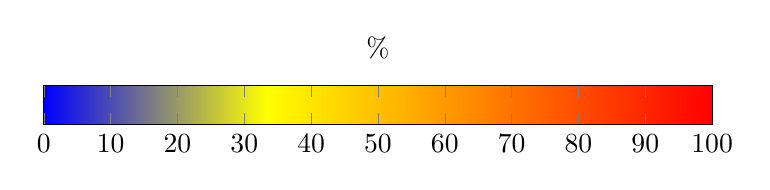
\begin{tikzpicture}
		\begin{axis}[
			hide axis,
			scale only axis,
			height=0pt,
			width=0pt,
			colormap/hot,
			colorbar horizontal,
			point meta min=0,
			point meta max=100,
			colorbar style={
				title=\%,
				width=0.7\textwidth,
				xtick={0, 10, 20, 30, 40, ..., 100}
			}]
			\addplot [draw=none] coordinates {(0,0)};
		\end{axis}
	\end{tikzpicture}
	\caption[Additive operators]{\textbf{Type distribution for additive operators} - Both operators are mainly used with the \textit{number-number} combination. Operator $+$ is also used for pure string concatenation. However, due to JS Type Coercion, $+$ is also used for \textit{string} and \textit{number} concatenation}
	\label{fig:experiments-additive-operators}
\end{figure}

\begin{figure}[tp]
	\centering

	\begin{tikzpicture}
		\begin{axis}[
			view={0}{90},
			title=Operator ${*}$,
			width=0.45\textwidth,
			colormap/hot,
			xticklabels={number,string,undefined,object,null,boolean,function,array},
			xtick={0,...,7},
			yticklabels={number,string,undefined,object,null,boolean,function,array},
			ytick={7,...,0},
			x tick label style={rotate=90,anchor=east}]
		]
		\addplot3[surf, shader=interp, left] file {figures/experiments/operators/multiplicative-operators/operator_star.dat};
		\end{axis}
	\end{tikzpicture}
	%
	\begin{tikzpicture}
		\begin{axis}[
			view={0}{90},
			width=0.45\textwidth,
			title=Operator ${/}$,
			colormap/hot,
			xticklabels={number,string,undefined,object,null,boolean,function,array},
			xtick={0,...,7},
			yticklabels={number,string,undefined,object,null,boolean,function,array},
			ytick={7,...,0},
			x tick label style={rotate=90,anchor=east}]
		\addplot3[surf, shader=interp, left] file {figures/experiments/operators/multiplicative-operators/operator_division.dat};
		\end{axis}
	\end{tikzpicture}

	\centering
	\begin{tikzpicture}
		\begin{axis}[
			view={0}{90},
			width=0.45\textwidth,
			title=Operator ${\%}$,
			colormap/hot,
			xticklabels={number,string,undefined,object,null,boolean,function,array},
			xtick={0,...,7},
			yticklabels={number,string,undefined,object,null,boolean,function,array},
			ytick={7,...,0},
			x tick label style={rotate=90,anchor=east}]
		\addplot3[surf, shader=interp, left] file {figures/experiments/operators/multiplicative-operators/operator_percentage.dat};
		\end{axis}
	\end{tikzpicture}
	
	\centering
	\hspace{0.1\textwidth}
	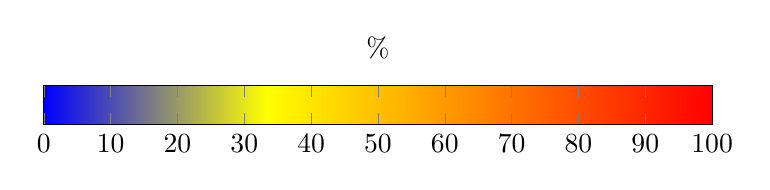
\begin{tikzpicture}
		\begin{axis}[
			hide axis,
			scale only axis,
			height=0pt,
			width=0pt,
			colormap/hot,
			colorbar horizontal,
			point meta min=0,
			point meta max=100,
			colorbar style={
				title=\%,
				width=0.7\textwidth,
				xtick={0, 10, 20, 30, 40, ..., 100}
			}]
			\addplot [draw=none] coordinates {(0,0)};
		\end{axis}
	\end{tikzpicture}
	\caption[Relational operators]{\textbf{Type distribution for multiplicative operators} - All multiplicative operators are mainly used with the \textit{number-number} combination}
\end{figure}

\begin{figure}[tp]
	\centering

	\begin{tikzpicture}
		\begin{axis}[
			view={0}{90},
			title=Operator ${==}$,
			width=0.45\textwidth,
			colormap/hot,
			xticklabels={number,string,undefined,object,null,boolean,function,array},
			xtick={0,...,7},
			yticklabels={number,string,undefined,object,null,boolean,function,array},
			ytick={7,...,0},
			x tick label style={rotate=90,anchor=east}]
		]
		\addplot3[surf, shader=interp, left] file {figures/experiments/operators/equality-operators/operator_==.dat};
		\end{axis}
	\end{tikzpicture}
	%
	\begin{tikzpicture}
		\begin{axis}[
			view={0}{90},
			width=0.45\textwidth,
			title=Operator ${!=}$,
			colormap/hot,
			xticklabels={number,string,undefined,object,null,boolean,function,array},
			xtick={0,...,7},
			yticklabels={number,string,undefined,object,null,boolean,function,array},
			ytick={7,...,0},
			x tick label style={rotate=90,anchor=east}]
		\addplot3[surf, shader=interp, left] file {figures/experiments/operators/equality-operators/operator_!=.dat};
		\end{axis}
	\end{tikzpicture}

	\centering
	\begin{tikzpicture}
		\begin{axis}[
			view={0}{90},
			width=0.45\textwidth,
			title=Operator ${===}$,
			colormap/hot,
			xticklabels={number,string,undefined,object,null,boolean,function,array},
			xtick={0,...,7},
			yticklabels={number,string,undefined,object,null,boolean,function,array},
			ytick={7,...,0},
			x tick label style={rotate=90,anchor=east}]
		\addplot3[surf, shader=interp, left] file {figures/experiments/operators/equality-operators/operator_===.dat};
		\end{axis}
	\end{tikzpicture}
	%
	\begin{tikzpicture}
		\begin{axis}[
			view={0}{90},
			width=0.45\textwidth,
			title=Operator ${!==}$,
			colormap/hot,
			xticklabels={number,string,undefined,object,null,boolean,function,array},
			xtick={0,...,7},
			yticklabels={number,string,undefined,object,null,boolean,function,array},
			ytick={7,...,0},
			x tick label style={rotate=90,anchor=east}]
		\addplot3[surf, shader=interp, left] file {figures/experiments/operators/equality-operators/operator_!==.dat};
		\end{axis}
	\end{tikzpicture}

	\centering
	\hspace{0.1\textwidth}
	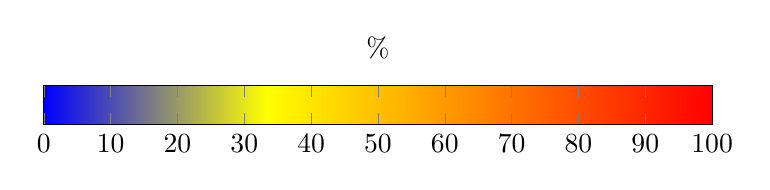
\begin{tikzpicture}
		\begin{axis}[
			hide axis,
			scale only axis,
			height=0pt,
			width=0pt,
			colormap/hot,
			colorbar horizontal,
			point meta min=0,
			point meta max=100,
			colorbar style={
				title=\%,
				width=0.7\textwidth,
				xtick={0, 10, 20, 30, 40, ..., 100}
			}]
			\addplot [draw=none] coordinates {(0,0)};
		\end{axis}
	\end{tikzpicture}
	\caption[Relational operators]{
		\textbf{Type distribution for equality operators} - Operator ${==}$ is mainly used for number comparison. String comparison is performed by using ${===}$ and ${!==}$ operators. Comparison against \textit{null} is performed by using both ${!=}$ and ${!==}$ operators
	}
	\label{fig:experiments-equality-operators}
\end{figure}

\begin{figure}[tp]
	\centering
	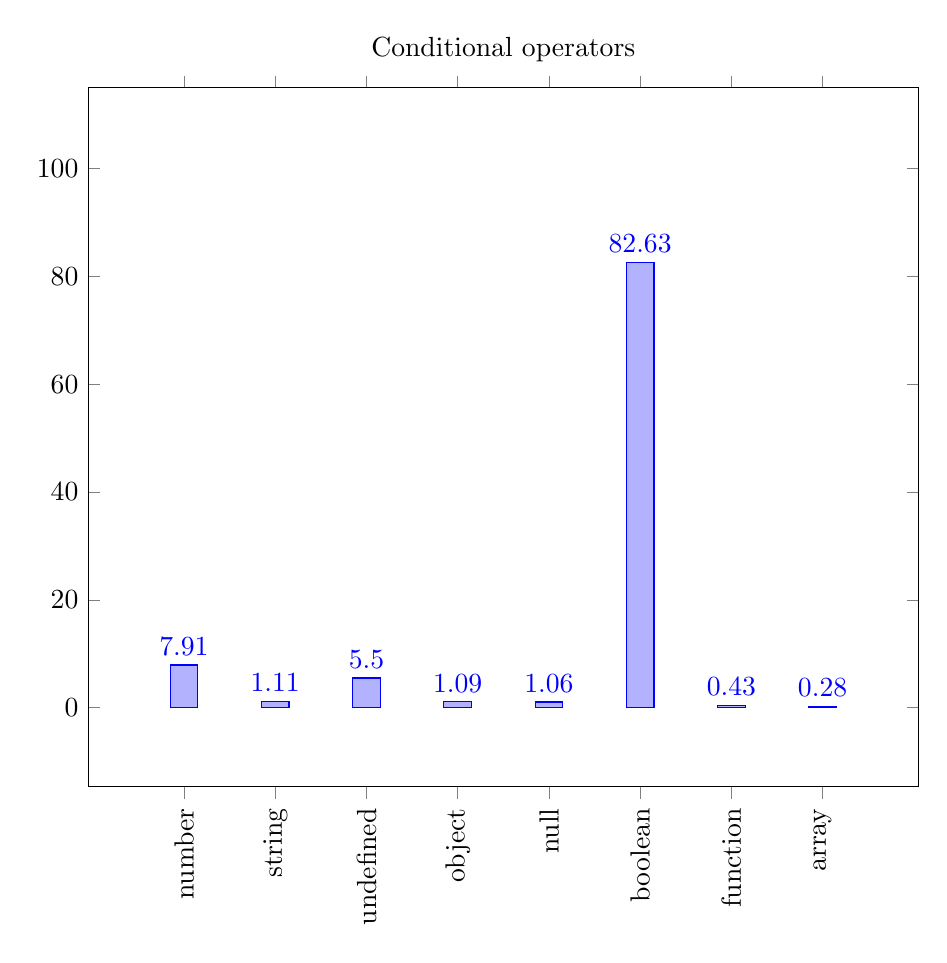
\begin{tikzpicture}
		\begin{axis}[
			ybar,
			title=Conditional operators,
			width=1\textwidth,
			ybar=0pt,
			ymax=100,
			enlargelimits=0.15,
			legend style={at={(0.5,-0.2)}, anchor=north,legend columns=-1},
			symbolic x coords={number,string,undefined,object,null,boolean,function,array},
			xtick=data,
			nodes near coords, 
			nodes near coords align={vertical},
			x tick label style={rotate=90,anchor=east},
		]
		\addplot coordinates {
			(number, 7.91)
			(string, 1.11)
			(undefined, 5.50)
			(object, 1.09)
			(null, 1.06)
			(boolean, 82.63)
			(function, 0.43)
			(array, 0.28)
		};
		\end{axis}
	\end{tikzpicture}
	\caption[Conditional operators]{\textbf{Type distribution for conditional operators} - It includes all operators that trigger a condition check before branching: ${if-then-else}$, ${switch-case}$, ${while}$, ${for}$, ${||}$, ${\&\&}$, ${ ? : }$.
	}
\end{figure}